\documentclass[14pt]{extbook}
\usepackage{multicol, enumerate, enumitem, hyperref, color, soul, setspace, parskip, fancyhdr} %General Packages
\usepackage{amssymb, amsthm, amsmath, bbm, latexsym, units, mathtools} %Math Packages
\everymath{\displaystyle} %All math in Display Style
% Packages with additional options
\usepackage[headsep=0.5cm,headheight=12pt, left=1 in,right= 1 in,top= 1 in,bottom= 1 in]{geometry}
\usepackage[usenames,dvipsnames]{xcolor}
\usepackage{dashrule}  % Package to use the command below to create lines between items
\newcommand{\litem}[1]{\item#1\hspace*{-1cm}\rule{\textwidth}{0.4pt}}
\pagestyle{fancy}
\lhead{Module7}
\chead{}
\rhead{Version A}
\lfoot{4758-2646}
\cfoot{}
\rfoot{testing}
\begin{document}

\begin{enumerate}
\litem{
Determine the domain of the function below.\[ f(x) = \frac{6}{15x^{2} +15 x -30} \]\begin{enumerate}[label=\Alph*.]
\item \( \text{All Real numbers except } x = a \text{ and } x = b, \text{ where } a \in [-19, -15] \text{ and } b \in [24, 27] \)
\item \( \text{All Real numbers except } x = a, \text{ where } a \in [-4, 0] \)
\item \( \text{All Real numbers except } x = a, \text{ where } a \in [-19, -15] \)
\item \( \text{All Real numbers except } x = a \text{ and } x = b, \text{ where } a \in [-4, 0] \text{ and } b \in [1, 4] \)
\item \( \text{All Real numbers.} \)

\end{enumerate} }
\litem{
Determine the domain of the function below.\[ f(x) = \frac{6}{20x^{2} +31 x + 12} \]\begin{enumerate}[label=\Alph*.]
\item \( \text{All Real numbers except } x = a \text{ and } x = b, \text{ where } a \in [-20.02, -19.99] \text{ and } b \in [-12.01, -11.97] \)
\item \( \text{All Real numbers except } x = a, \text{ where } a \in [-20.02, -19.99] \)
\item \( \text{All Real numbers except } x = a \text{ and } x = b, \text{ where } a \in [-0.81, -0.77] \text{ and } b \in [-0.79, -0.7] \)
\item \( \text{All Real numbers except } x = a, \text{ where } a \in [-0.81, -0.77] \)
\item \( \text{All Real numbers.} \)

\end{enumerate} }
\litem{
Solve the rational equation below. Then, choose the interval(s) that the solution(s) belongs to.\[ \frac{-7x}{2x -3} + \frac{-2x^{2}}{8x^{2} +2 x -21} = \frac{5}{4x + 7} \]\begin{enumerate}[label=\Alph*.]
\item \( x \in [-2.68,-1.86] \)
\item \( x_1 \in [-0.08, 0.28] \text{ and } x_2 \in [-4.5,1.2] \)
\item \( \text{All solutions lead to invalid or complex values in the equation.} \)
\item \( x_1 \in [-0.08, 0.28] \text{ and } x_2 \in [1.3,4] \)
\item \( x \in [-1.96,-1.47] \)

\end{enumerate} }
\litem{
Choose the graph of the equation below.\[ f(x) = \frac{1}{x - 3} - 2 \]\begin{enumerate}[label=\Alph*.]
\begin{multicols}{2}\item 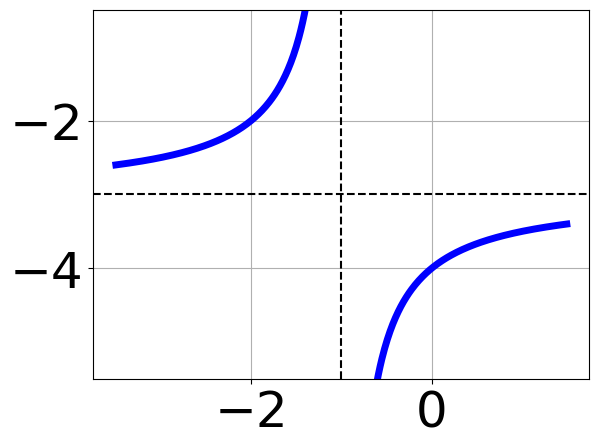
\includegraphics[width = 0.3\textwidth]{../Figures/rationalEquationToGraphAA.png}\item 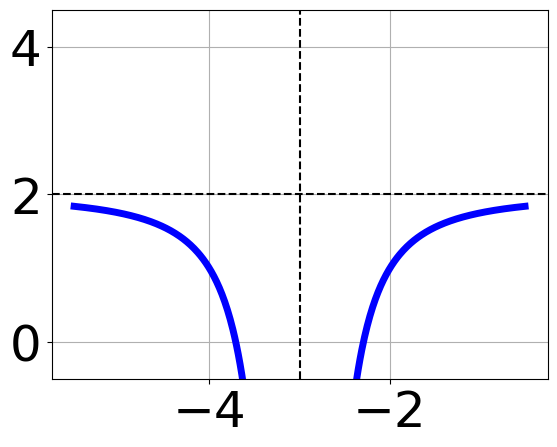
\includegraphics[width = 0.3\textwidth]{../Figures/rationalEquationToGraphBA.png}\item 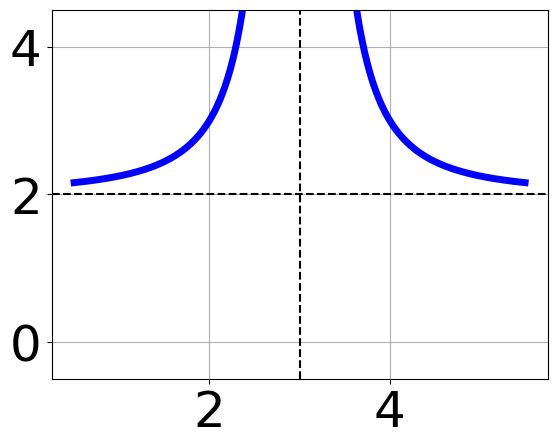
\includegraphics[width = 0.3\textwidth]{../Figures/rationalEquationToGraphCA.png}\item 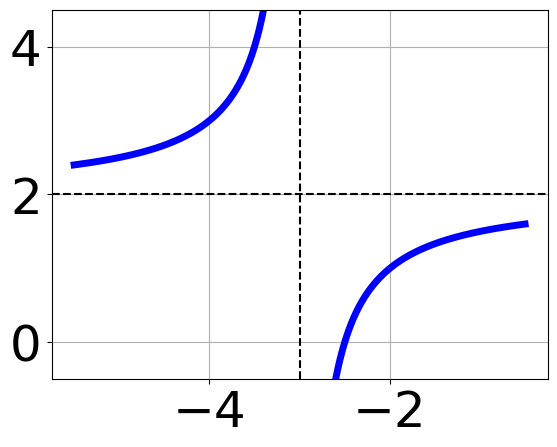
\includegraphics[width = 0.3\textwidth]{../Figures/rationalEquationToGraphDA.png}\end{multicols}\item None of the above.
\end{enumerate} }
\litem{
Choose the graph of the equation below.\[ f(x) = \frac{-1}{x - 2} + 3 \]\begin{enumerate}[label=\Alph*.]
\begin{multicols}{2}\item 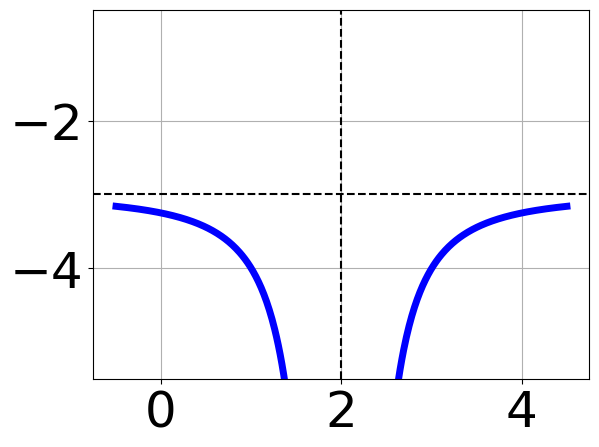
\includegraphics[width = 0.3\textwidth]{../Figures/rationalEquationToGraphCopyAA.png}\item 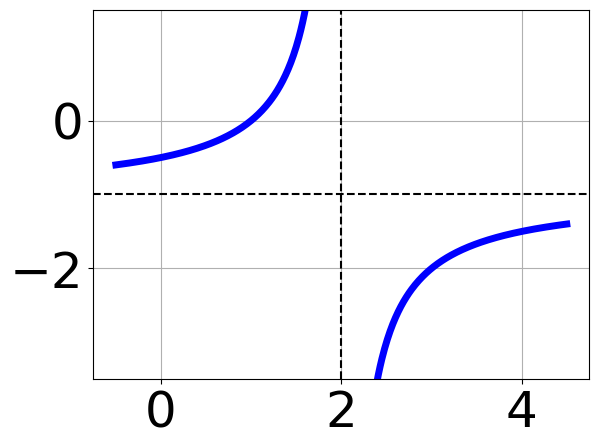
\includegraphics[width = 0.3\textwidth]{../Figures/rationalEquationToGraphCopyBA.png}\item 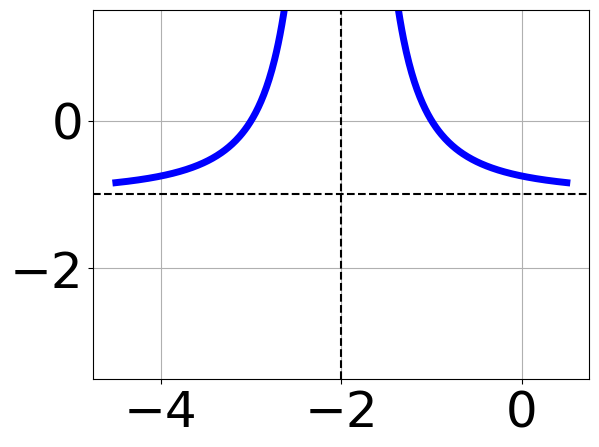
\includegraphics[width = 0.3\textwidth]{../Figures/rationalEquationToGraphCopyCA.png}\item 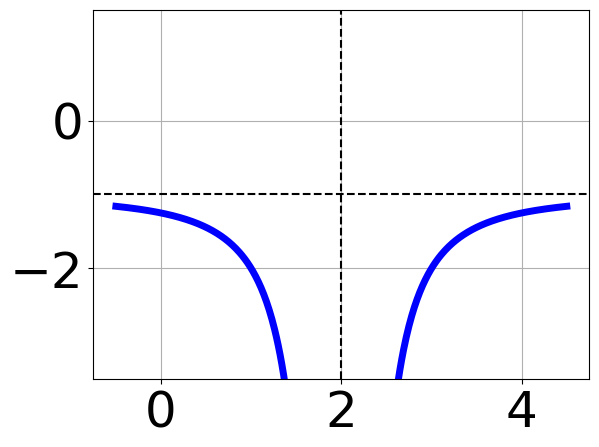
\includegraphics[width = 0.3\textwidth]{../Figures/rationalEquationToGraphCopyDA.png}\end{multicols}\item None of the above.
\end{enumerate} }
\litem{
Choose the equation of the function graphed below.
\begin{center}
    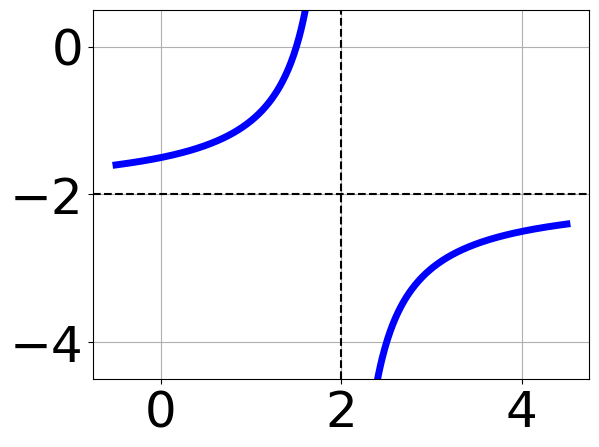
\includegraphics[width=0.5\textwidth]{../Figures/rationalGraphToEquationCopyA.png}
\end{center}
\begin{enumerate}[label=\Alph*.]
\item \( f(x) = \frac{1}{(x + 2)^2} - 2 \)
\item \( f(x) = \frac{-1}{x - 2} - 2 \)
\item \( f(x) = \frac{1}{x + 2} - 2 \)
\item \( f(x) = \frac{-1}{(x - 2)^2} - 2 \)
\item \( \text{None of the above} \)

\end{enumerate} }
\litem{
Solve the rational equation below. Then, choose the interval(s) that the solution(s) belongs to.\[ \frac{6}{8x + 2} + -2 = \frac{-8}{-72x -18} \]\begin{enumerate}[label=\Alph*.]
\item \( \text{All solutions lead to invalid or complex values in the equation.} \)
\item \( x_1 \in [-0.28, 0.41] \text{ and } x_2 \in [0.45,0.6] \)
\item \( x \in [0.39,1.43] \)
\item \( x_1 \in [-0.28, 0.41] \text{ and } x_2 \in [0.61,0.73] \)
\item \( x \in [0.07,2.07] \)

\end{enumerate} }
\litem{
Solve the rational equation below. Then, choose the interval(s) that the solution(s) belongs to.\[ \frac{-26}{91x + 78} + 1 = \frac{-26}{91x + 78} \]\begin{enumerate}[label=\Alph*.]
\item \( x \in [-0.14,1.86] \)
\item \( x \in [-1.86,0.14] \)
\item \( x_1 \in [-3.86, 0.14] \text{ and } x_2 \in [-0.4,1] \)
\item \( \text{All solutions lead to invalid or complex values in the equation.} \)
\item \( x_1 \in [-3.86, 0.14] \text{ and } x_2 \in [-1.8,0.1] \)

\end{enumerate} }
\litem{
Solve the rational equation below. Then, choose the interval(s) that the solution(s) belongs to.\[ \frac{-4x}{3x + 5} + \frac{-6x^{2}}{-9x^{2} -33 x -30} = \frac{2}{-3x -6} \]\begin{enumerate}[label=\Alph*.]
\item \( x_1 \in [-0.23, 0.72] \text{ and } x_2 \in [-2.67,0.33] \)
\item \( x \in [-5.8,-2.34] \)
\item \( \text{All solutions lead to invalid or complex values in the equation.} \)
\item \( x_1 \in [-0.23, 0.72] \text{ and } x_2 \in [-5.48,-2.48] \)
\item \( x \in [-2.32,-1.28] \)

\end{enumerate} }
\litem{
Choose the equation of the function graphed below.
\begin{center}
    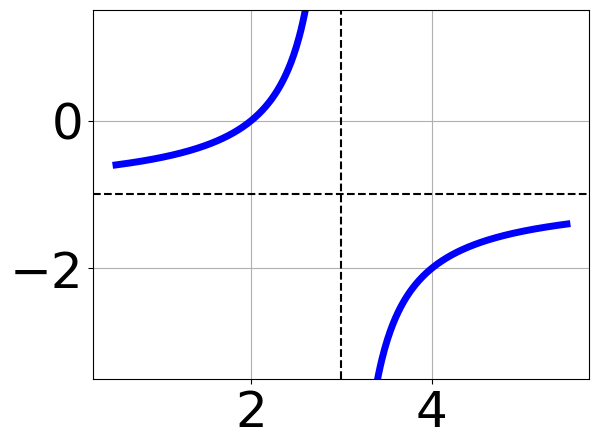
\includegraphics[width=0.5\textwidth]{../Figures/rationalGraphToEquationA.png}
\end{center}
\begin{enumerate}[label=\Alph*.]
\item \( f(x) = \frac{1}{x + 3} - 2 \)
\item \( f(x) = \frac{-1}{x - 3} - 2 \)
\item \( f(x) = \frac{-1}{(x - 3)^2} - 2 \)
\item \( f(x) = \frac{1}{(x + 3)^2} - 2 \)
\item \( \text{None of the above} \)

\end{enumerate} }
\end{enumerate}

\end{document}